	%%%%%%%%%%%%%%%%%%%%%%%%%%%%%%%%%%%%%%%%%%%%%%%%%%%%%%%%%%%%%%%%%%%%%%%%%%%
%%  esrel2025-paper.tex   :   19/12/2018 			                     %%
%%  Text file to use with rps-esrel2023. written in Latex2e.             %%
%%  The content, structure, format and layout of this style file is the  %%
%%  property of Research Publishing Services                             %%
%%  Copyright (c) 2011-2023 Research Publishing Services,                %%
%%  All rights are reserved.                                             %%
%%%%%%%%%%%%%%%%%%%%%%%%%%%%%%%%%%%%%%%%%%%%%%%%%%%%%%%%%%%%%%%%%%%%%%%%%%%

\documentclass[twocolumn]{rps-esrel2026}
%\documentclass[draft, twocolumn]{rps-esrl2026} 

\def\papername{\jobname}

\def\ds{\displaystyle}


%\usepackage[authoryear]{biblatex-chicago}

\usepackage{natbib}
\usepackage{adjustbox}
%\usepackage[authoryear]{natbib}

\begin{document}

\markboth{Temitope Ohiani, Caroline Pyke and Edoardo Patelli}{Information Propagation and Network Analysis in Directed Acyclic Networks: A web interface}

%%%%%%%%%%%%%%%%%%%%%%%%% Plase keep this command for single column for abstract section.
\twocolumn[
%%%%%%%%%%%%%%%%%%%%%%%%%

\title{A no-code web interface for Reliability Analysis in Directed Acyclic Networks}

\author{Temitope Ohiani }

\address{Department of Civil and Environmental Engineering, University of Strathclyde, UK. \email{temitope.ohiani@strath.ac.uk}}


\author{Caroline Pyke}

\address{United Kingdom National Nuclear Laboratory, UK. \email{caroline.pyke@uknnl.com}}

\author{Edoardo Patelli}
\address{Department of Civil and Environmental Engineering, University of Strathclyde, UK. \email{edoardo.patelli@strath.ac.uk}}

\begin{abstract}
Domain experts in infrastructure, reliability, and systems engineering often need advanced analytical tools to assess networked systems under uncertainty, but many available methods remain inaccessible because they require programming expertise and fragmented software workflows. This creates a persistent “last-mile” gap between algorithm development and practical use.

This paper presents a local-first, no-code web interface for information propagation and network analysis in directed acyclic networks. Built on the \texttt{InformationPropagationAnalysis.jl} Julia package, the system provides an interactive visual environment for network construction and inspection, subgraph decomposition, exact reachability analysis, uncertainty-aware propagation, capacity assessment, and time- and cost-based path analysis. The software adopts a decoupled architecture, with a Julia computational back-end and an Angular browser-based front-end, both running entirely on the user’s local machine. This preserves data sovereignty while supporting modular extension and testing.

The functionality of the interface is demonstrated on the WATER wastewater treatment benchmark under seven operational scenarios, including both deterministic and interval-valued inputs. The results show how the interface supports rapid comparative analysis across scenarios without requiring users to write code or move data to external services.
\end{abstract}

\keywords{Network Analysis, Information Propagation, Directed Acyclic Networks, System Reliability, Web Interface, Julia.}

%%%%%%%%%%%%%%%%%%%%%%%%% Please keep this closing bracket to complete the single column format for abstract.
]
%%%%%%%%%%%%%%%%%%%%%%%%%

\section{Introduction}
From design through operation and maintenance, decision makers need tools that can both represent the structure of complex systems and quantify how resources, signals, or constraints propagate through them. Graph-based methods have long provided a natural framework for this purpose in civil infrastructure, logistics, reliability engineering, and interconnected systems. The mathematical tools for probabilistic reasoning, uncertainty representation, and network performance analysis are well established \cite{pearl1988probabilistic,koller2009probabilistic,ferson2013}. 
Unfortunately, it is well known that the people who need these tools most are rarely the developers of these tools. 
Domain experts often understand their systems in detail but lack the programming expertise required to use many existing analytical tools effectively. Sometimes described as the ``last mile problem'', studies consistently report this gap between algorithmic availability and practical adoption~\cite{hannay2009scientists, prabhu2011survey}.

In recent years, several tools have been developed with the goal of making network analysis more accessible, though many of these solutions only address part of the problem. For example, network visualization tools such as Gephi~\cite{bastian2009gephi} and Cytoscape~\cite{shannon2003cytoscape} offer an interactive environment for graph construction and rendering but they do not support any analytical work. These tools usually have to be combined with domain-specific software which often comes with its own data format requirements and a learning curve that can be steep for users that are not familiar with the algorithms.

In many network-based reliability problems, data on component failure rates or link transmission probabilities can be sparse, incomplete, or derived from expert judgement, and require the right tool to fully capture dependency information. Although packages and libraries supporting probabilistic reasoning have been developed for Matlab \cite{OpenCossan}, R~\cite{ferson2019pbar}, Julia~\cite{gray2022pba_julia}, and Python~\cite{gray2022pba}, users wishing to use these methods must be prepared to write code directly against these libraries.

In many cases, no single tool covers both the structural and quantitative aspects of an assessment. Accessibility requirements further reduce the pool of available tools. As a result, complete system profiling often requires combining several of these tools, transforming data between them and managing multiple separate workflows.

Deployment architecture is another important factor that impacts the likelihood of adoption and accessibility of new scientific software. The local-first movement~\cite{kleppmann2019local} encourages the development of software that prioritizes user data sovereignty while maintaining collaborative features. Although cloud-based solutions can be convenient, they raise data sovereignty and privacy concerns~\cite{hashizume2013analysis} that often prevent their use in industries with proprietary data (such as nuclear and defence).

To date, no existing tool offers a fully visual interface that combines structural and quantitative network analysis with native uncertainty quantification while running entirely on the user's local machine. This paper addresses this gap by presenting a local-first web interface that combines visual network modelling and quantitative analysis for directed acyclic networks in a single no-code workflow.


\section{System Architecture and Analysis Framework}

\subsection{Local architecture}
As illustrated in Figure~\ref{fig:architecture}, the web interface follows a client-server pattern where both the back-end and the front-end run on the user's local machine. This architecture separates the computational back-end (developed in Julia) from the interactive browser-based environment (written in Angular). This allows each side to be extended, tested, and deployed independently. 


From the user's perspective, this separation is largely transparent:  the browser-based interface communicates with the local analytical engine  through HTTP requests on \texttt{localhost}. This design preserves usability while allowing the computational engine and interface layer to evolve independently..

For developers and technical researchers, this already removes the need to reimplement these algorithms from scratch, since the exposed functions can be called directly and the package can be extended or overridden as needed. However, the majority of excluded users are not looking to write code at all.

Domain experts who understand the implications of an analysis and know how to make decisions from results are often not programmers. The web interface was developed for these users.

\begin{figure*}[t]
    \centering
    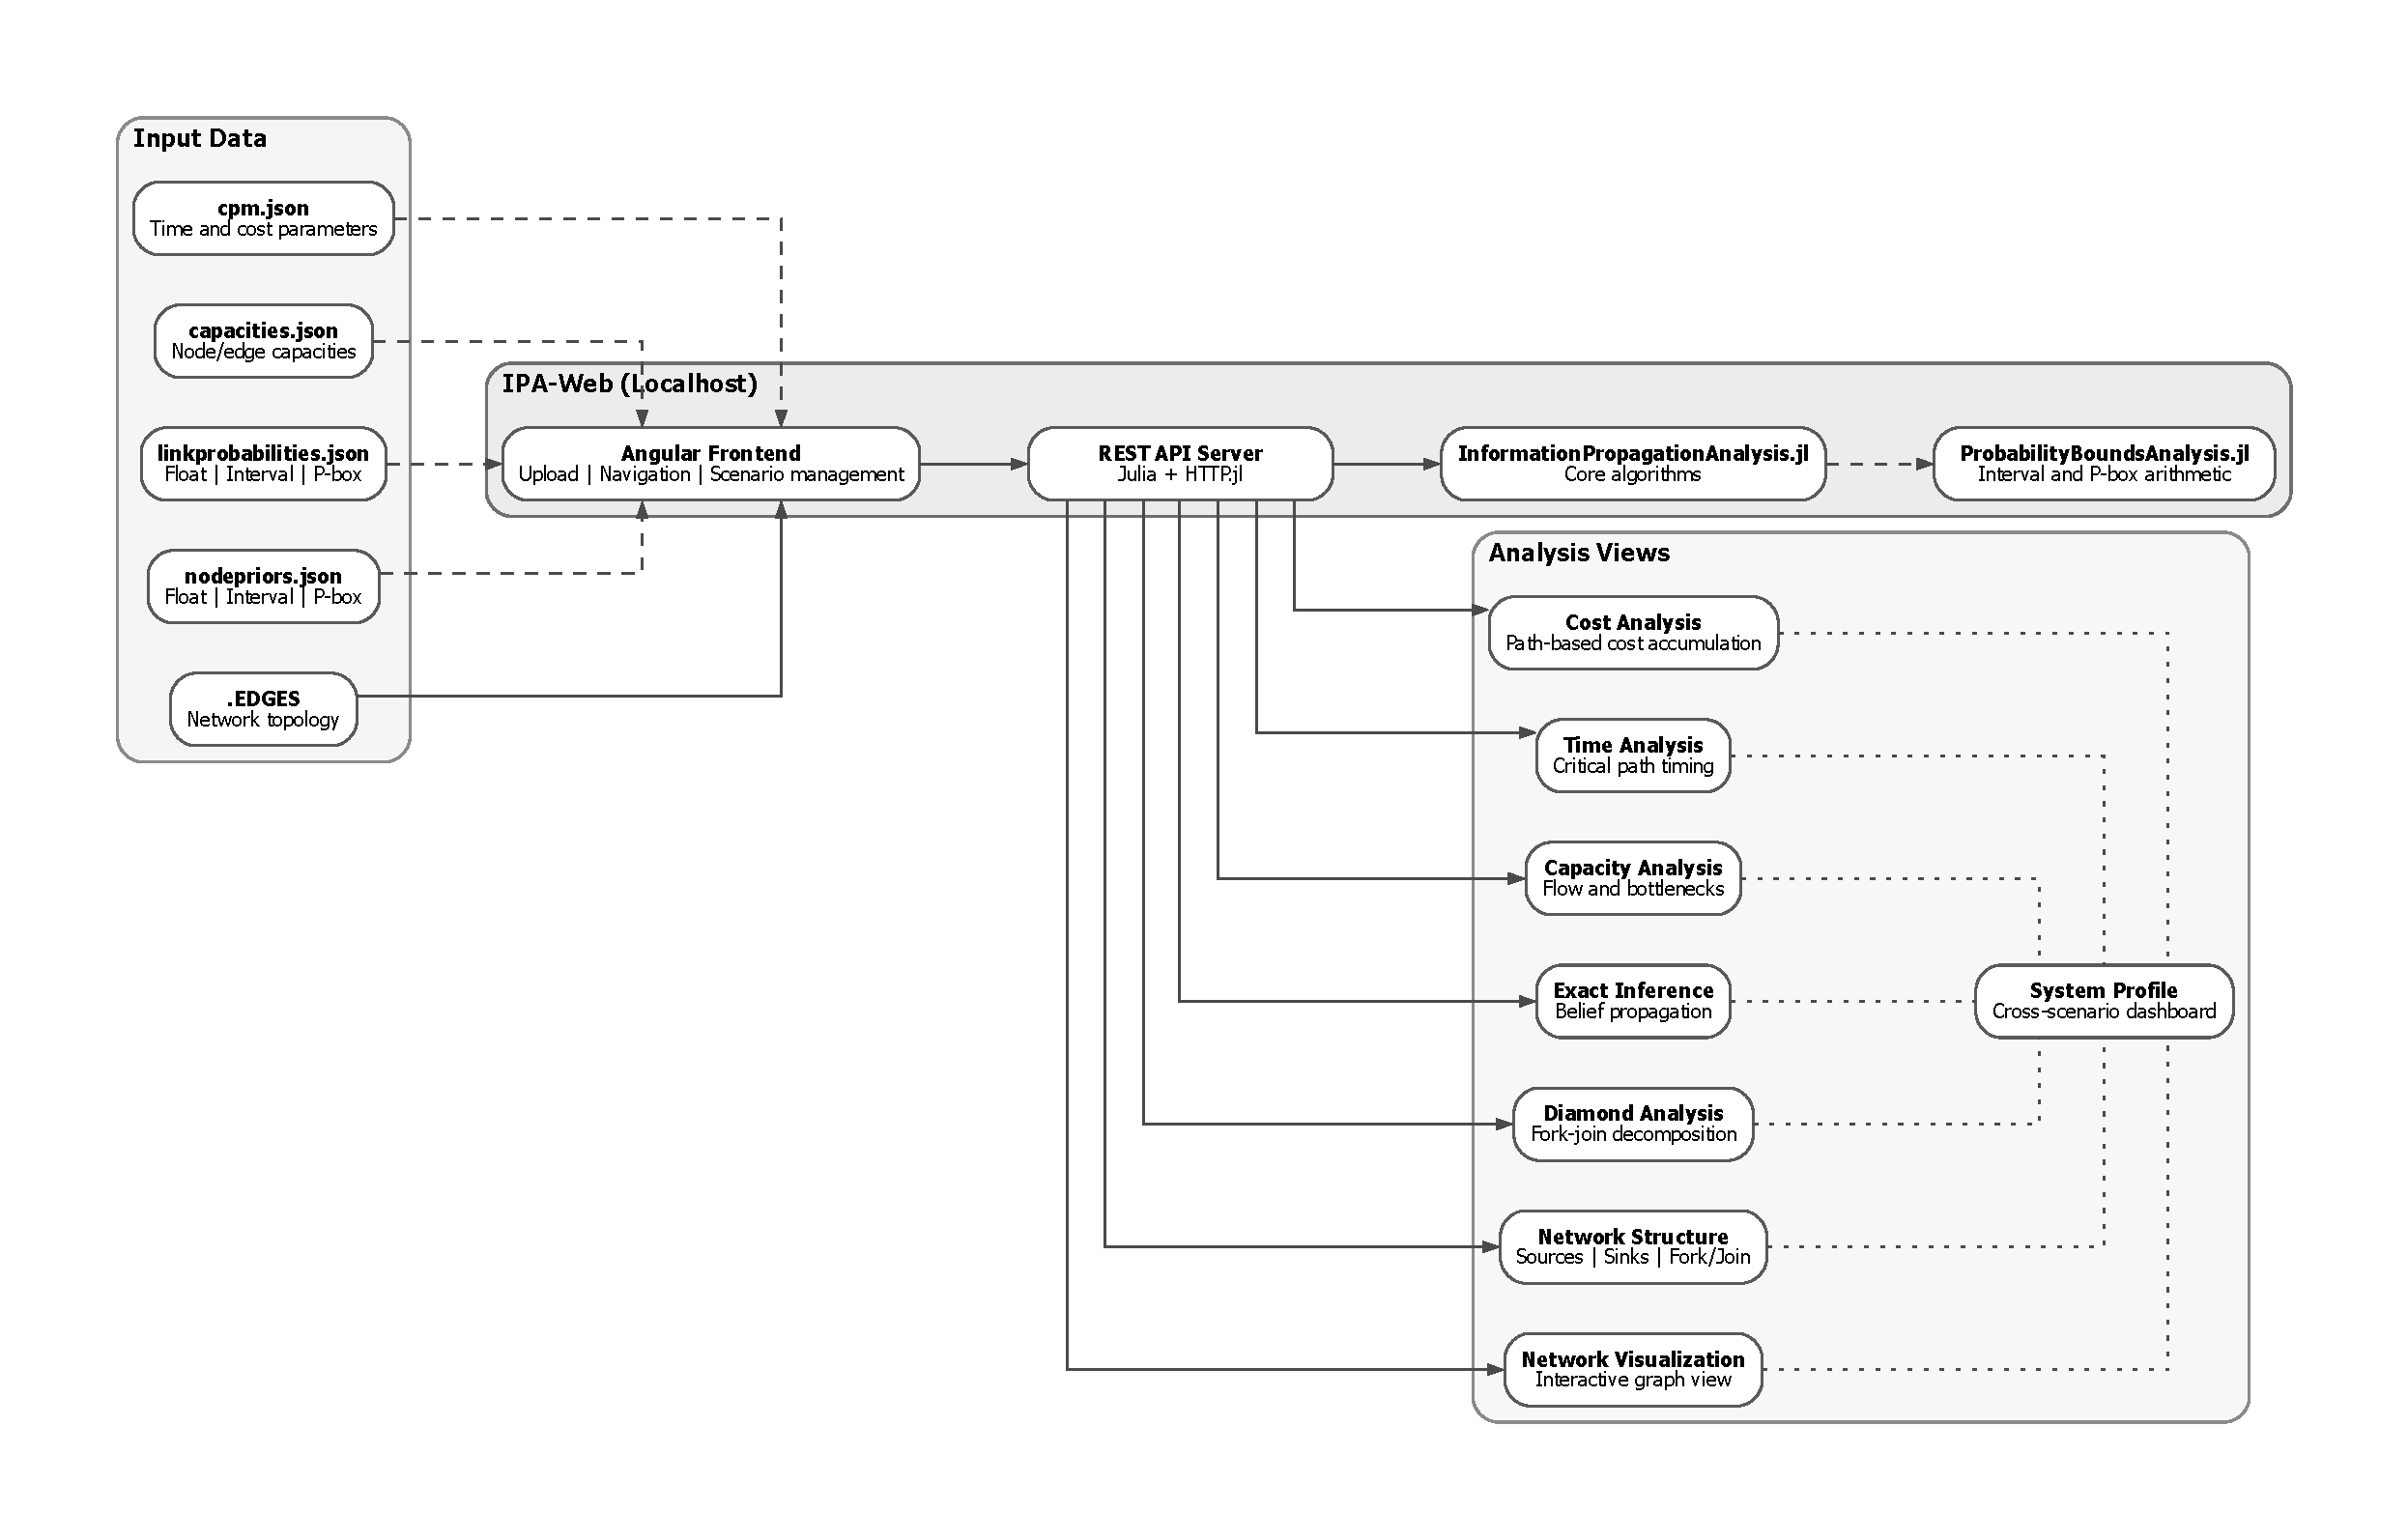
\includegraphics[height=0.45\textheight,width=\textwidth,keepaspectratio]{images/architecture_paper.pdf}
    
    \caption{The IPA-Web decoupled software architecture}
    \label{fig:architecture}
\end{figure*}

\subsection{Available analysis capabilities}
Built around a Julia computational back-end and an Angular front-end, the \texttt{InformationPropagationAnalysis.jl} the \texttt{InformationPropagationAnalysis.jl} package~\cite{infoprop2026_julia} provides a multi-algorithm framework for analysing directed acyclic graph (DAG) networks.

The framework is made up of five modules. 

The \textbf{Input Processing Module} serves as the main entry point to the framework. It parses raw network data, adjacency information, probabilities, capacities, and time or cost attributes, and transforms them into an enriched graph object. This object stores both the network structure and precomputed information such as topological order and ancestor/descendant relations, enabling efficient downstream analysis and interactive inspection in the interface (Fig.~\ref{fig:ui_structure_combo}a).


\begin{figure*}[t]
    \centering
    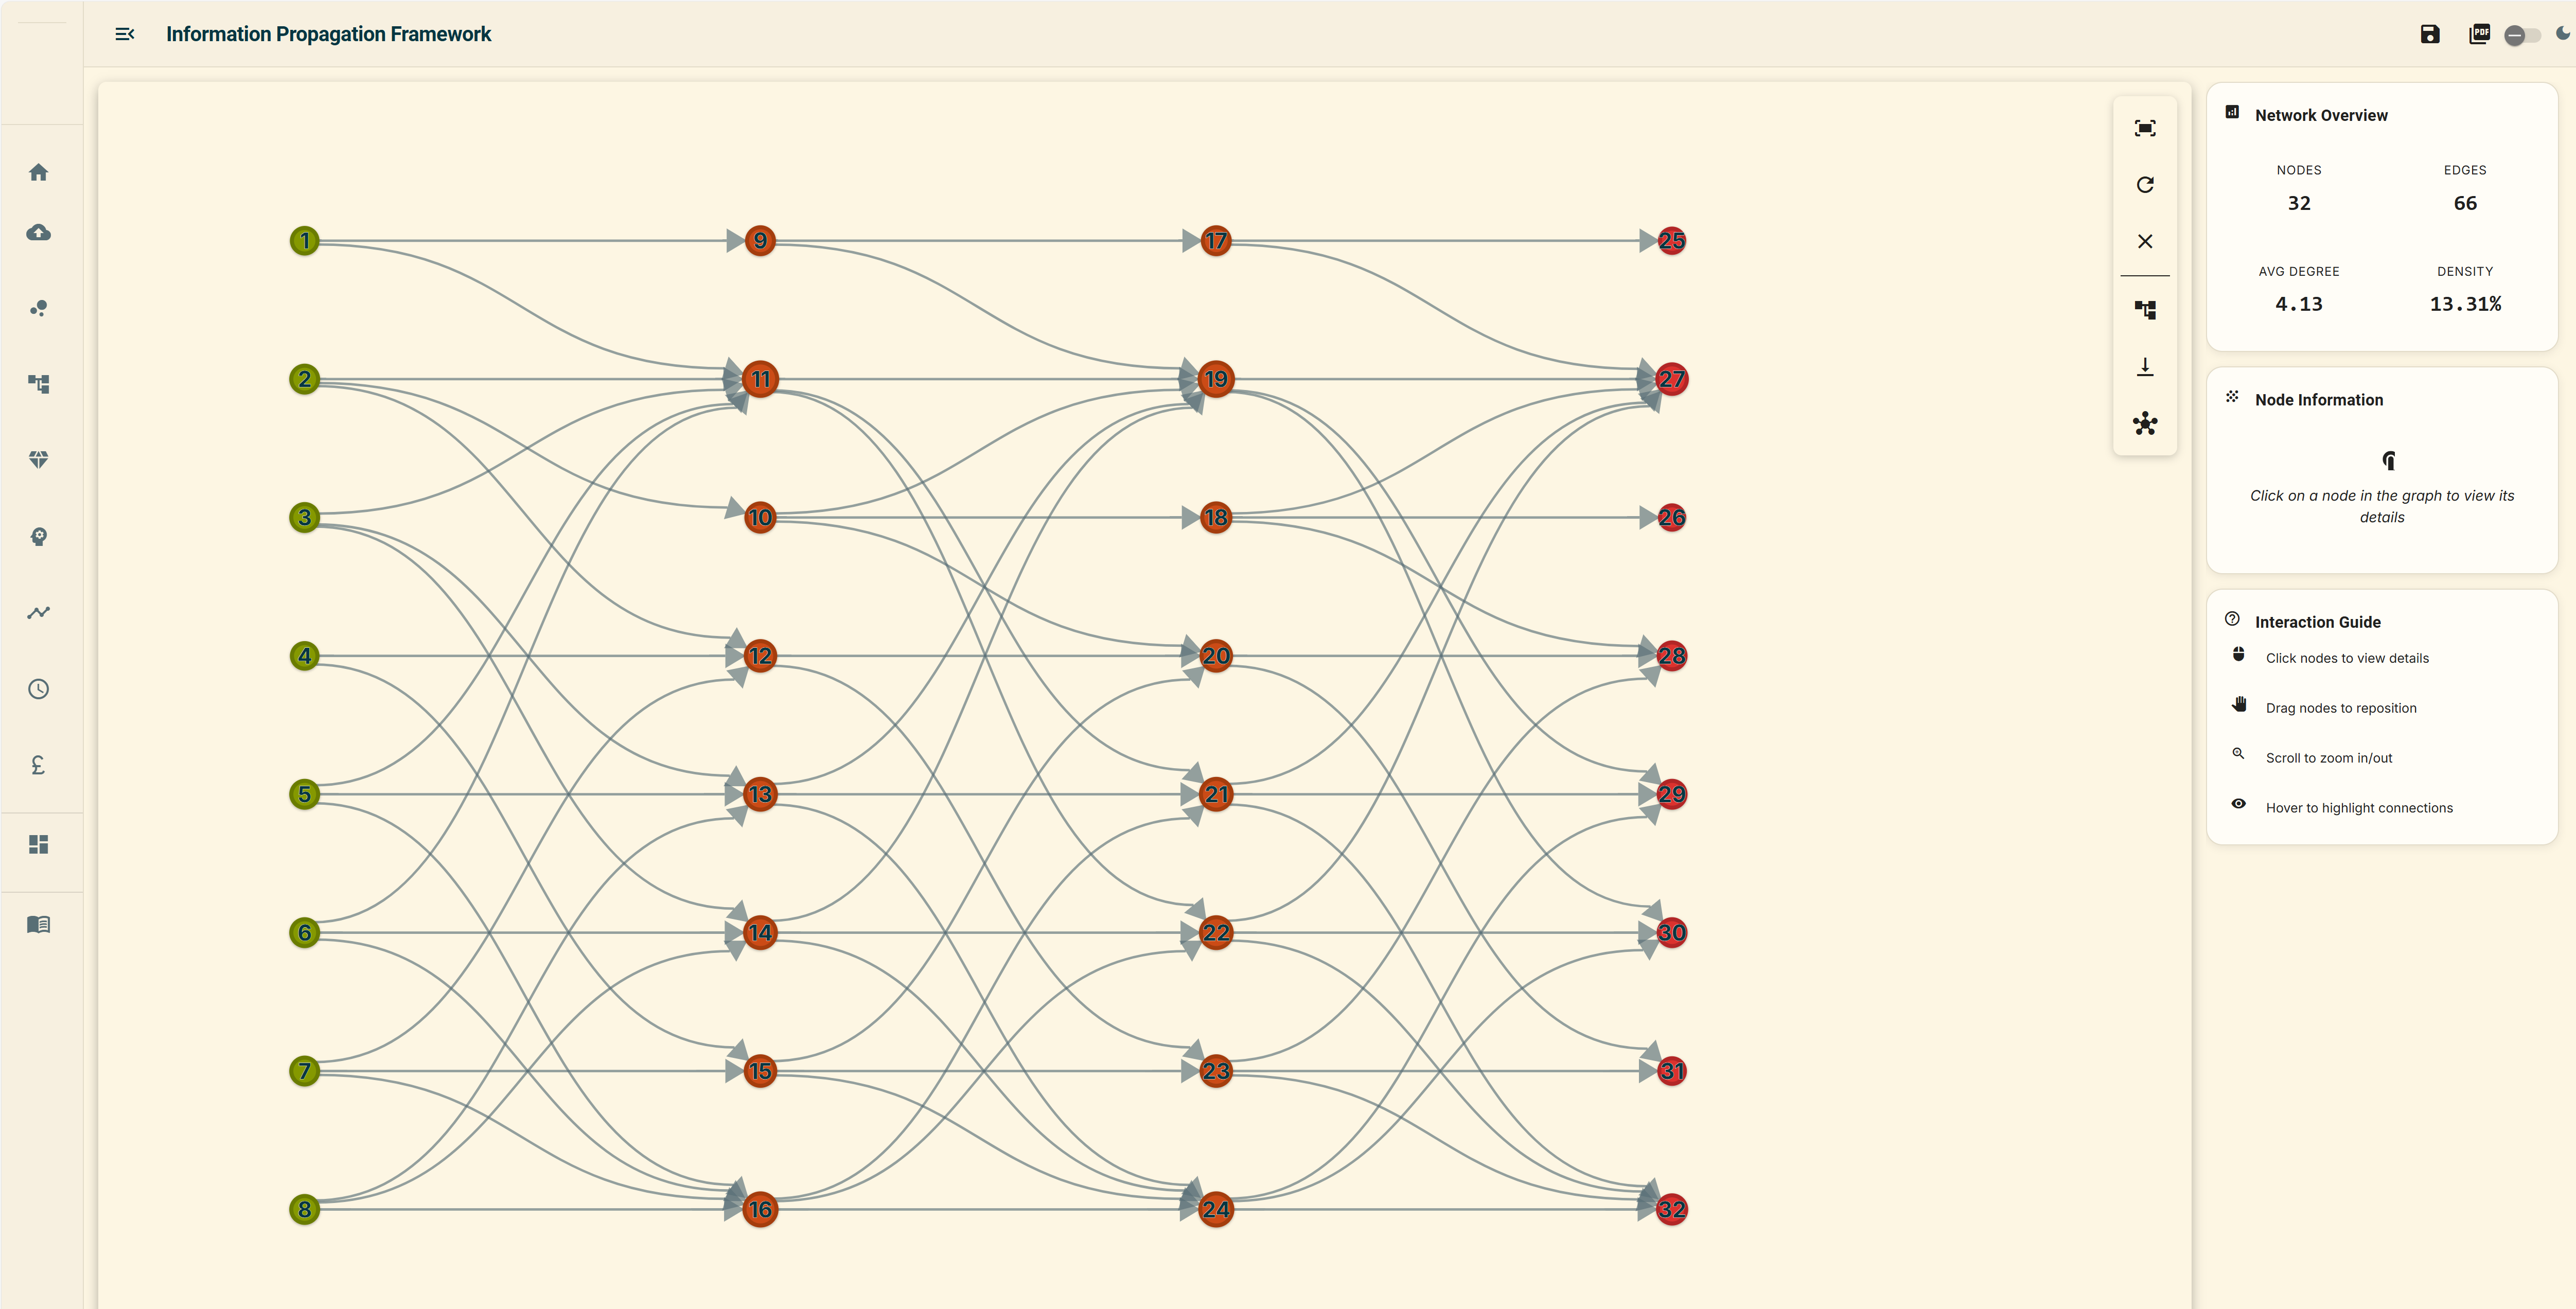
\includegraphics[height=\textheight,width=0.9\linewidth,keepaspectratio]{images/network-visuliation.png}
    
    \vspace{0.5cm}
    
    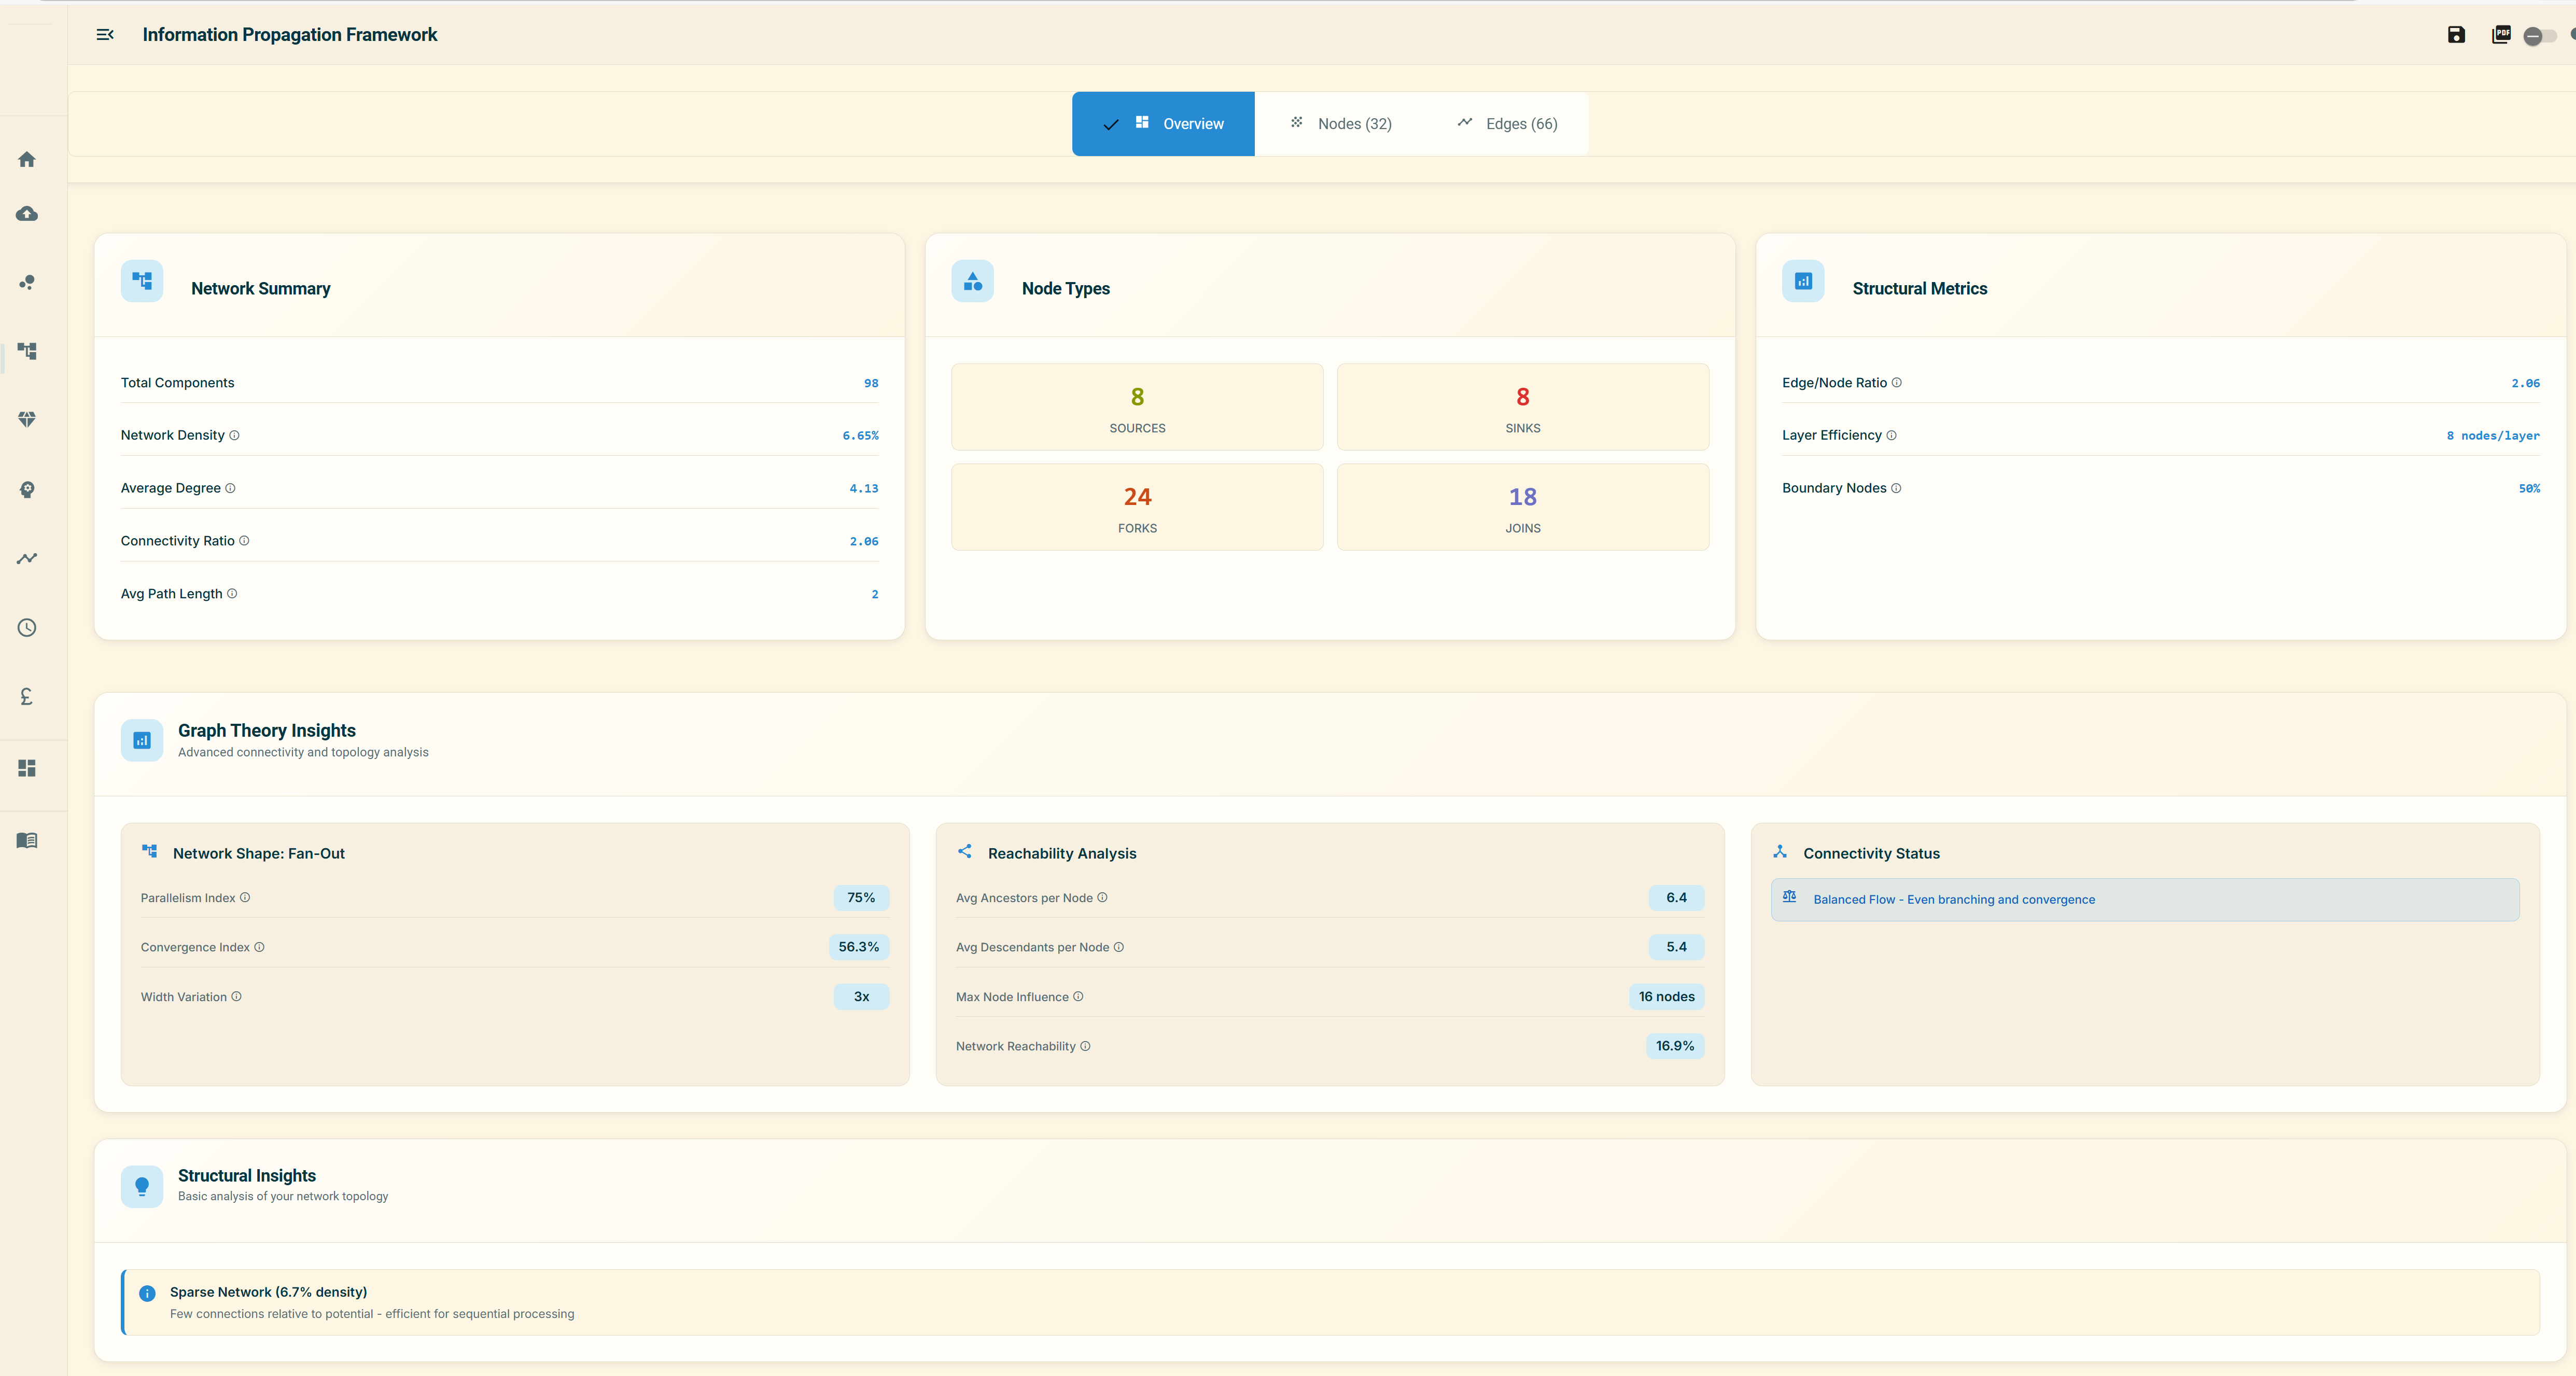
\includegraphics[height=\textheight,width=0.9\linewidth,keepaspectratio]{images/network-structure-view.png}
    
    \caption{Combined graph object view: (a) interactive network visualization and (b) network structure dashboard.}
    \label{fig:ui_structure_combo}
\end{figure*}

The \textbf{Subgraph Decomposition Module} detects fork--join subgraphs, in particular diamond structures within the enriched DAG.. In real infrastructure processes, "diamond"-like subgraphs are formed when two or more distinct paths diverge from shared upstream nodes $f_1, \ldots, f_k$ and later re-converge at a downstream join node $j$ that is a descendant of those same shared nodes.

The detection algorithm performs an exhaustive search for all possible diamonds in the network. For optimal traversal, the topological sort from the global graph object drives the discovery order. This order naturally builds a cache of already-discovered diamonds that is drawn on when building and resolving overlapping and nested structures. The sorting ensures that all diamond patterns in the network are processed in a single pass, even when the same previously discovered diamond appears later in the context of a larger diamond.

The advantages of precomputing these subgraphs and their equivalent dependency structures become even more apparent in other modules that employ statistical conditioning and causal reasoning, because the dependency information is already resolved before propagation begins rather than having to be rediscovered and compiled every time a node has diamonds in its ancestry, which in large and dense networks can be costly. Beyond conditional probabilities, the unique diamond objects themselves are stored as the same type of graph object and can therefore be used for isolated or focused evaluation without needing to run a solution on the full network. As with all other modules, the decomposition module is designed to be extendable, so that other subgraph types beyond diamonds can be defined if needed.


The \textbf{Reachability Module} evaluates, for each node in the DAG, the probability that at least one active path reaches it from the source nodes. Depending on the application, node and edge probabilities may represent transmission success, operational availability, or reliability. The module implements the IPA reachability algorithm for exact propagation in directed acyclic networks, with conditional handling of reconvergent diamond structures. The node reliability at each node $n$ is computed as:

For each node $n$, the algorithm computes the probability (e.g. reliability, reachability) that at least one active path reaches $n$:
\begin{equation}\label{eq:belief}
R(n) = \pi(n) \cdot P\!\left(\text{at least one working path reaches  } n\right)
\end{equation}
where $\pi(n)$ is the node prior. For a node with parents $p_1, \ldots, p_k$, the ``at least one path'' probability uses inclusion-exclusion:
\begin{equation}\label{eq:inclexcl}
P\!\Bigl(\bigcup_{i=1}^{k} A_i\Bigr) = \sum_{j=1}^{k} (-1)^{j+1} \!\!\sum_{|I|=j} \prod_{i \in I} S_i
\end{equation}
where $S_i = R(p_i) \cdot \ell(p_i, n)$ is the signal through parent $p_i$ and edge probability $\ell(p_i, n)$. For diamond joins, the algorithm conditions on all $2^k$ states of the shared ancestors:
\begin{equation}\label{eq:diamond_cond}
R(j) = \sum_{\mathbf{s} \in \{0,1\}^k} P(\mathbf{s}) \cdot P(j \mid \mathbf{s})
\end{equation}

The message passing sequence follows the topological sort inherited from the input module, and the full algorithmic details are described in detail in ~\cite{infoprop2026} and ~\cite{infoprop2026_julia}. For networks with diamond subgraphs, the causal boundaries through which shared causes must be conditioned can be read directly from those precomputed structures from the decomposition algorithm. Since data quality in real applications is often uneven, by default the BP algorithm supports fixed point values, intervals, and probability boxes (p-boxes) probabilistic data. 
Currently, the module does not support mixed input types within a single run since the input format is expected to match the output format. For mixed probability node and edge information, users may need to standardise their data beforehand. For algorithmic confidence, the module also exposes a full path enumeration method and a Monte Carlo implementation that can be run as independent validation against the algorithm’s results.

Whilst the reachability module answers probabilistic questions about the network, decision makers typically require additional metrics to build a complete system profile. The framework therefore includes two utility modules that extend the probability-based reasoning with capacity and scheduling analysis. In contrast to the belief propagation algorithm, whose cost depends on the number of conditioning nodes in diamond subgraphs (Eq.~\ref{eq:diamond_cond}), both utility modules operate in a single topological pass over the network, requiring $O(|V| + |E|)$ time. For most practical networks, this corresponds to near real-time computation.

The \textbf{Capacity Analysis Module} computes the maximum flow capacity of the network given node capacities, edge capacities, and source input rates. For each non-source node $n$, the sustainable flow is

\begin{equation}\label{eq:maxflow}
F(n) = \min\!\left(\sum_{p \in \mathrm{pa}(n)}
\min\bigl(F(p),\, c_{p \to n}\bigr),\; c_n\right).
\end{equation}

Here $F(p)$ denotes the flow at parent $p$, $c_{p \to n}$ the edge capacity, and $c_n$ the node processing capacity. Beyond maximum flow estimation, the module can identify bottleneck nodes or edges that restrict throughput and determine the widest path, defined as the path whose minimum capacity is maximal from source to target. It also reports overall network throughput as the ratio of total flow reaching target nodes to the total source input rate, providing a direct measure of how effectively the network delivers available input. 

In the interface, this allows users to identify bottlenecks, compare flow-limited scenarios, and trace critical operational dependencies without exporting the network to a separate optimisation tool.

The \textbf{Critical Path Module} serves as a generalized propagation engine where user can decide on the combination function $\bigoplus$,  edge propagation function $f$, and node function $g$. For each non-source node, the resulting value is

\begin{equation}\label{eq:cpm}
V(n) = g\!\left(\bigoplus_{p \in \mathrm{pa}(n)} f\bigl(V(p),\, w_{p \to n}\bigr),\; w_n\right).
\end{equation}

For instance, when $\bigoplus = \max$ and both $f$ and $g$ are additive, Eq.~(\ref{eq:cpm}) reduces to the standard critical path method, and $V(n)$ represents the earliest completion time at node $n$. Setting $\bigoplus = \min$ yields a bottleneck analysis, whereas choosing $\bigoplus = \sum$ produces cost accumulation along paths. Because the module treats these functions as parameters, a single implementation supports multiple analysis types within the same solution.

This enables users to switch between scheduling, bottleneck, and cumulative-cost views within the same interface and network model.

\section{Application Example: WATER  (Wastewater Treatment benchmark)} 
The interface is demonstrated using the WATER benchmark~\cite{water_benchmark}, a Bayesian wastewater treatment network frequently used to test algorithms on directed acyclic graphs. With 32 nodes and 66 directed edges  and an average Markov blanket size of 7.69, the network is compact enough to visualise clearly while still exhibiting the layered dependency structure and fork--join patterns relevant to the present framework.
More importantly, WATER's internal organization mirrors patterns we often see in real infrastructure systems. It's built from four repeated processing blocks, with dependencies that cross between layers. This creates fork--join patterns at multiple scales, exactly the kind of diamond subgraphs the decomposition module is designed to handle. The layered flow also lets us show how constraints ripple forward through consecutive stages, which is central to capacity analysis in sequential processes. Figure~\ref{fig:ui_structure_combo} shows how users first encounter the network: (a) presents the interactive visual graph object, while (b) summarizes its structural properties once loaded.

\begin{figure*}[p]
    \centering
    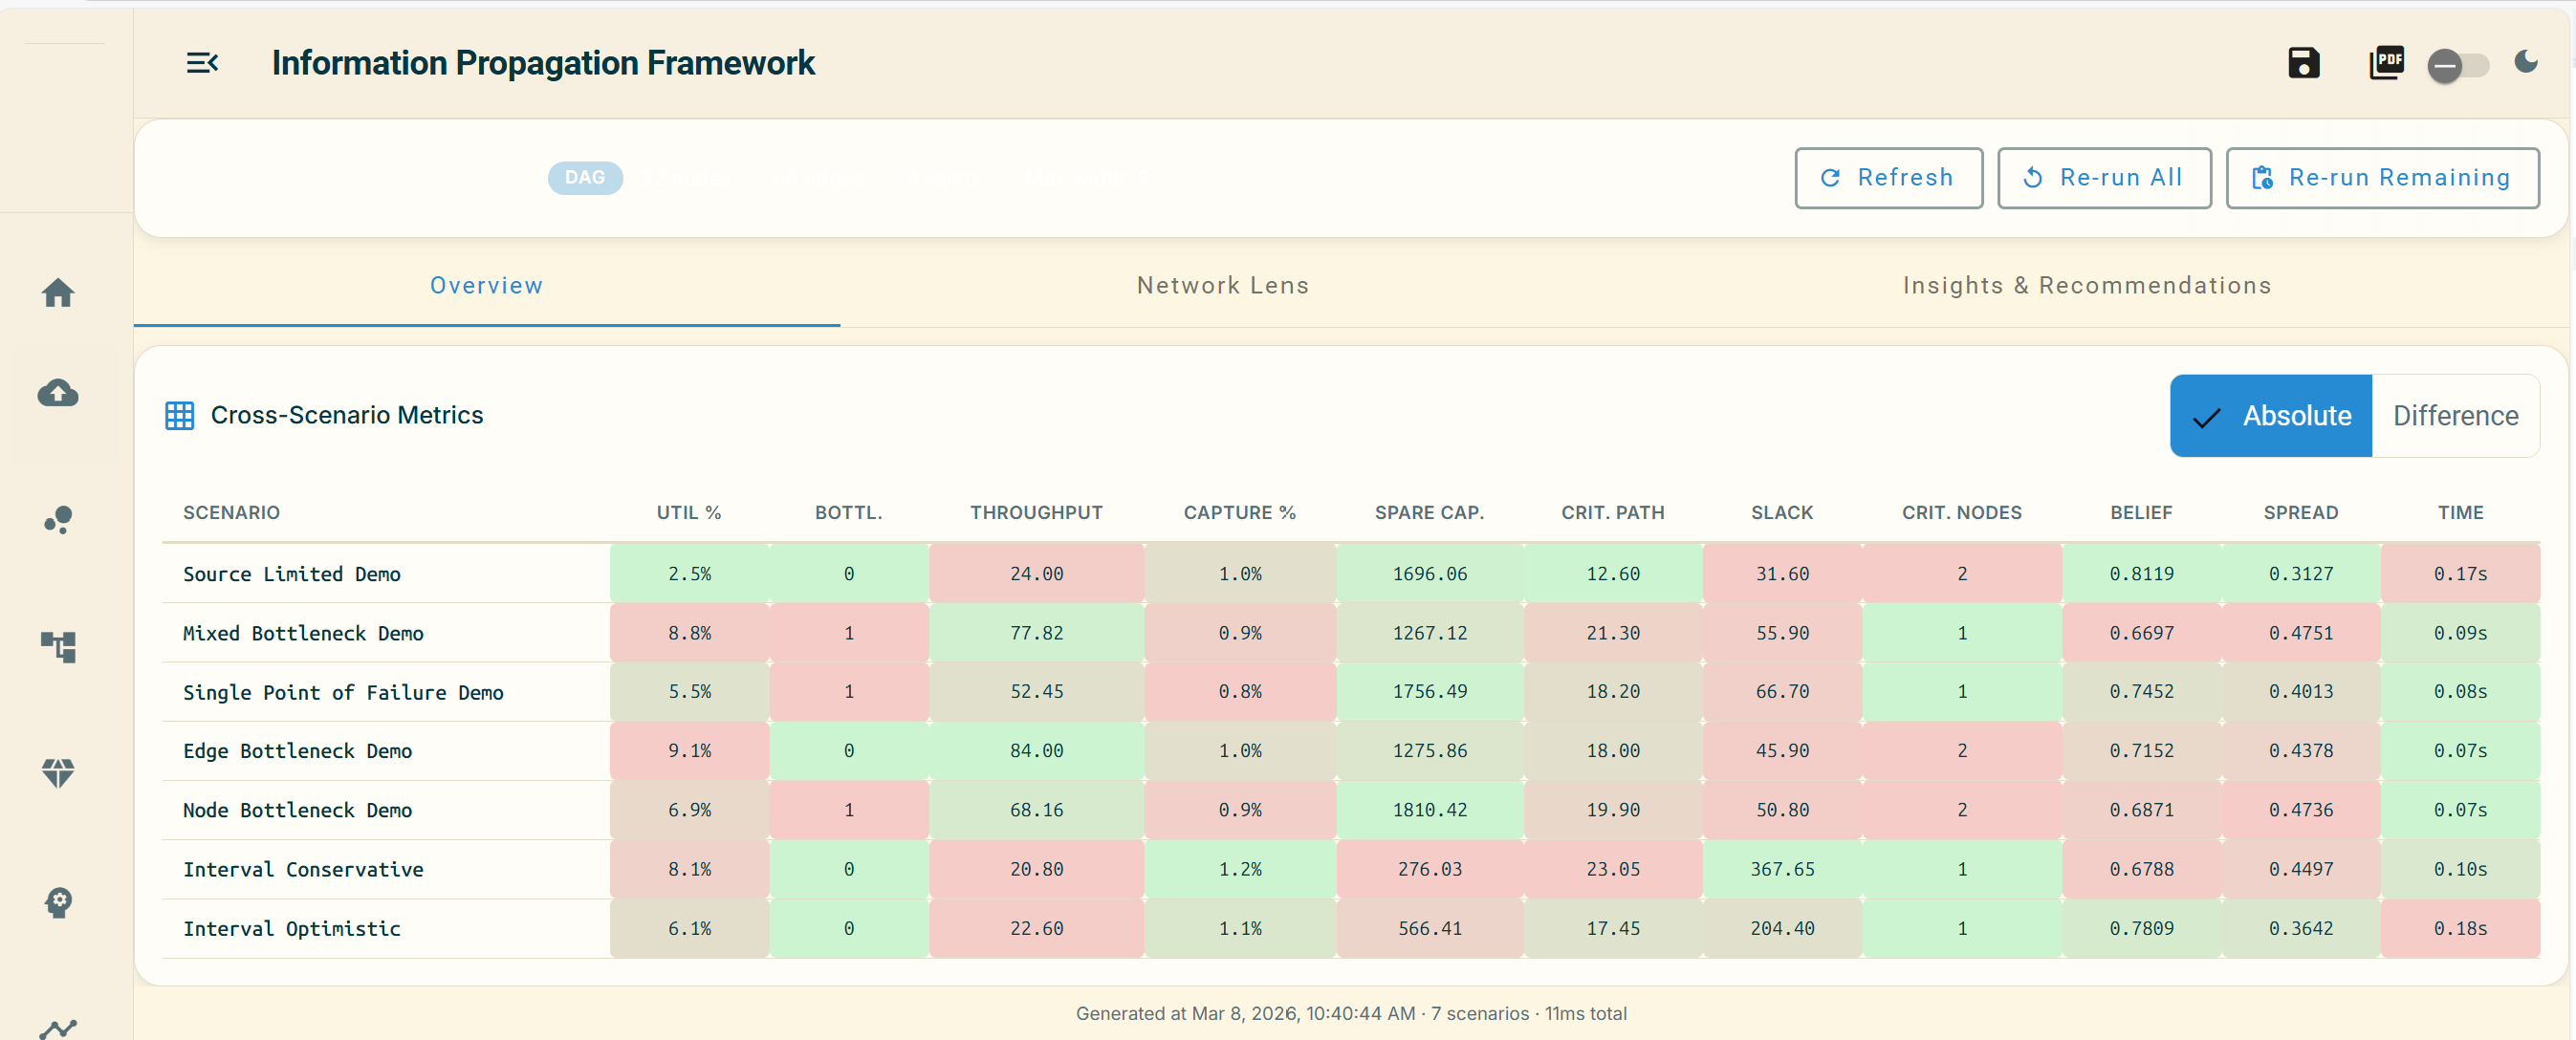
\includegraphics[width=\textwidth,height=0.22\textheight]{images/profile-ovrview.png}
    
    \vspace{0.2em}
    
    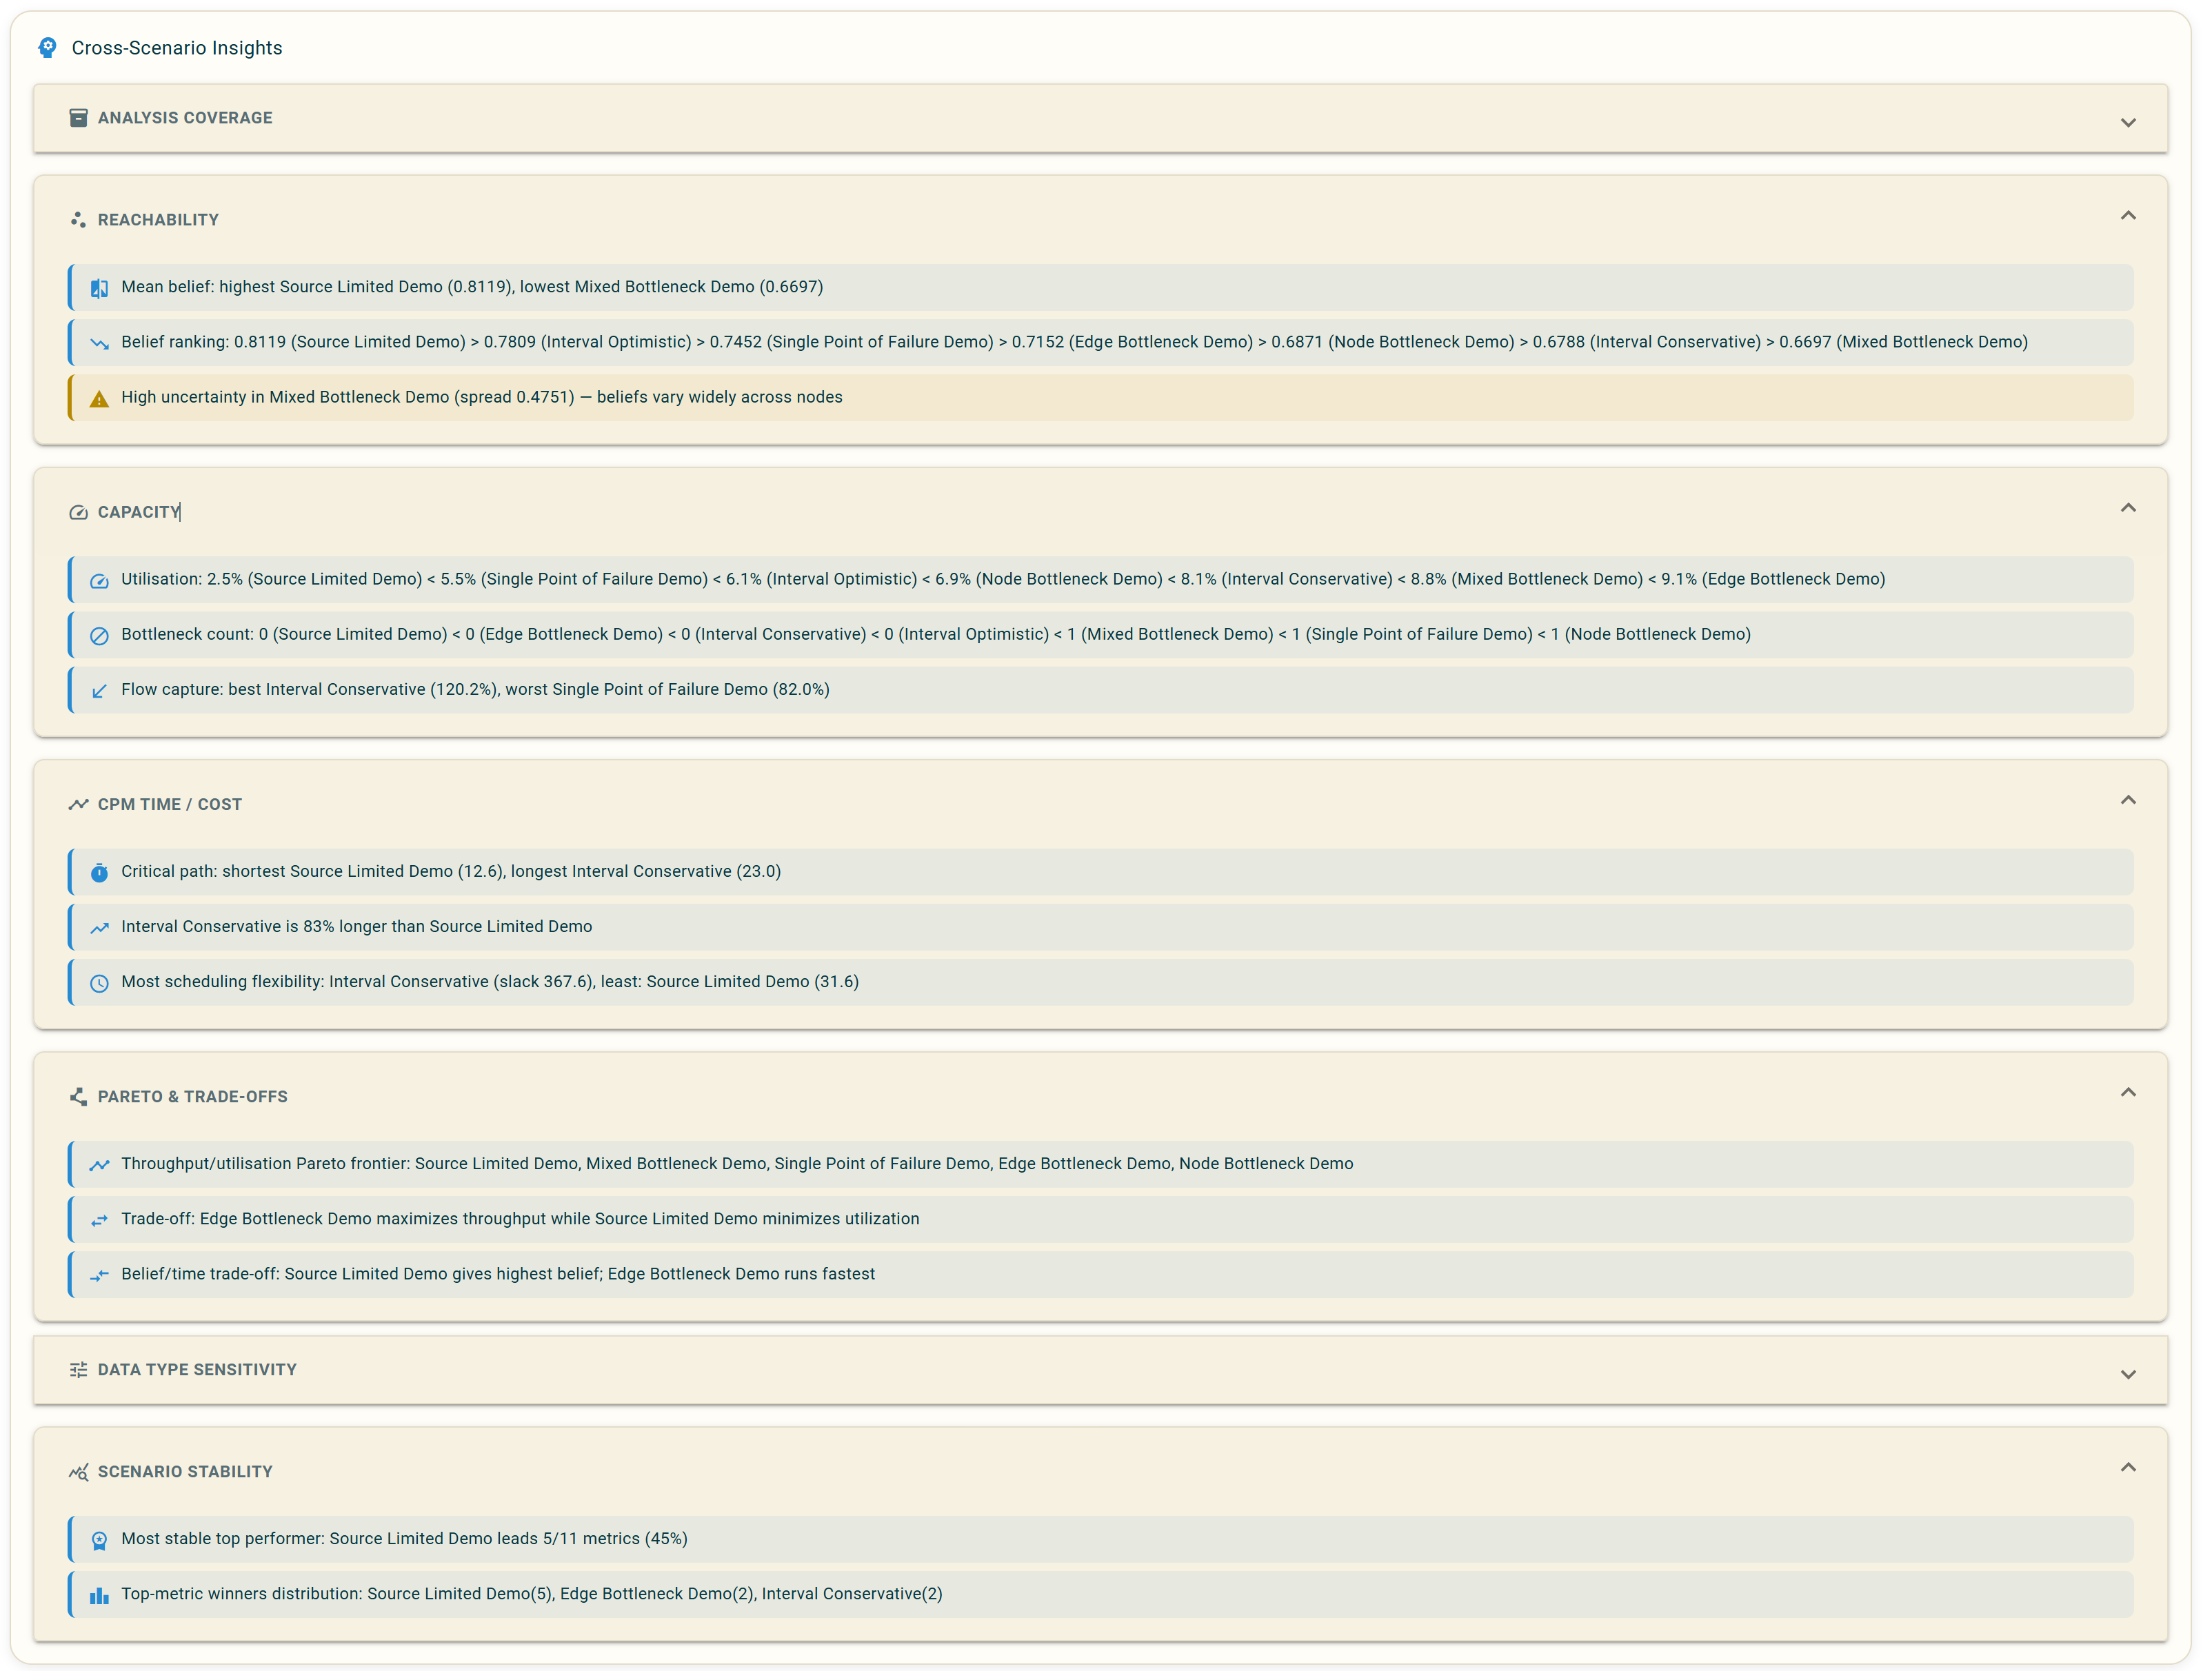
\includegraphics[width=\textwidth,height=0.35\textheight]{images/profile-insights.png}
    
    \vspace{0.2em}
    
    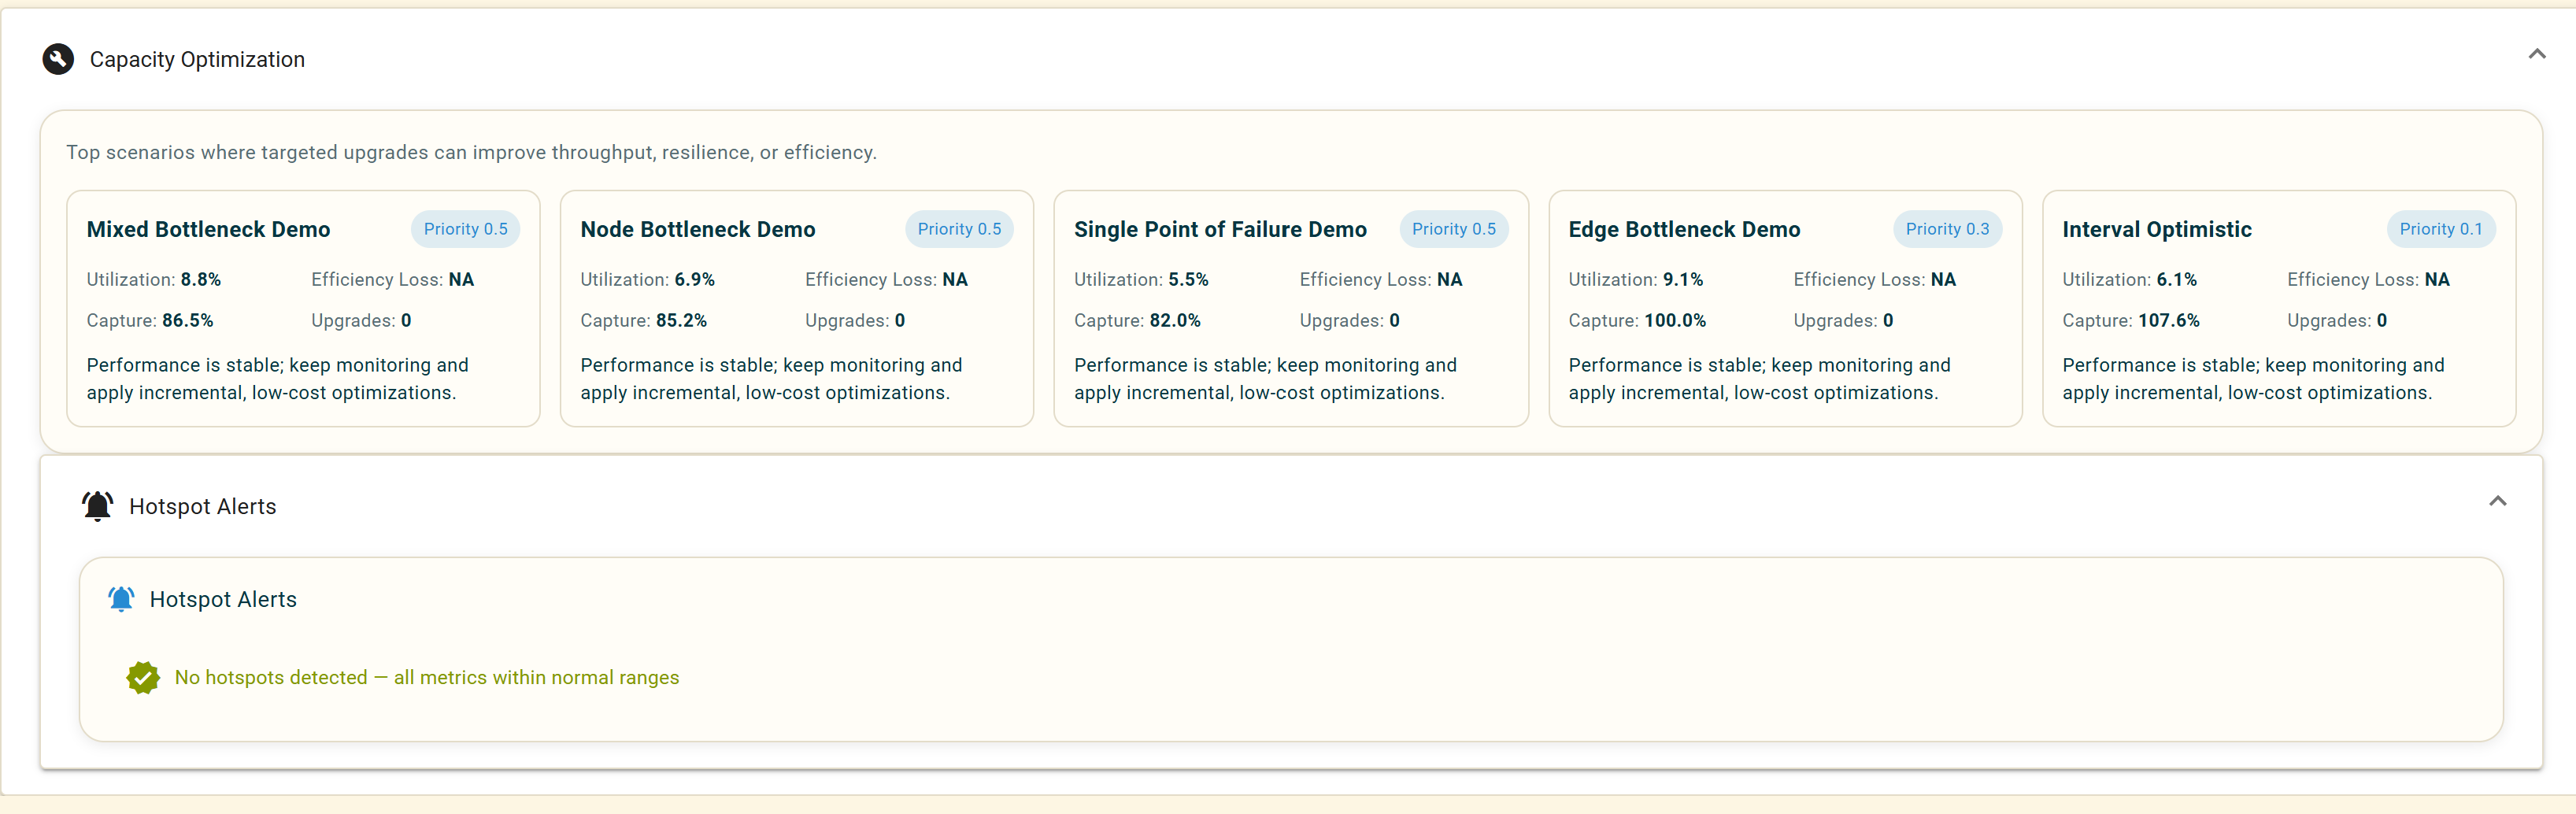
\includegraphics[width=\textwidth,height=0.28\textheight]{images/profile-optimization.png}
    
    \caption{System Profile dashboard: (top) cross-scenario overview, (middle) profile insights for decision support, (bottom) optimization recommendations.}
    \label{fig:profile_combo}
\end{figure*}

\subsection{Scenario design and walkthrough}\label{sec1}
Rather than test the system on a single configuration, seven operational scenarios were defined to explore different flow and failure regimes. Five use deterministic inputs to isolate specific bottleneck behaviours: \textit{Edge Bottleneck} restricts transmission capacity while leaving node processing unconstrained; \textit{Node Bottleneck} does the opposite. \textit{Mixed Bottleneck} imposes both types of constraints simultaneously, revealing how they compound. \textit{Source Limited} tests a system where internal capacity is plentiful but input supply falls short. \textit{Single Point of Failure} forces most flow through a critical hub, stressing the network's resilience when redundancy is removed.

The last two scenarios shift from point estimates to interval bounds. \textit{Interval Conservative} applies worst-case parameter values, while \textit{Interval Optimistic} uses best-case bounds. This distinction is important because real assessments rarely rely on perfectly known parameters. Operators often need to understand not only nominal performance but also the range of plausible outcomes under uncertainty.

After running the available analyses across all seven scenarios, users can compare the results through the System Profile dashboard (Figure~\ref{fig:profile_combo}). The overview panel summarises key metrics such as bottlenecks and critical paths, the insights panel highlights decision-relevant patterns, and the optimisation panel presents potential improvement actions. This consolidated view supports rapid cross-scenario comparison without requiring users to switch tools or manually aggregate results. The full interface is available on the framework's GitHub page~\cite{infoprop2026_julia}.



\section{Conclusions}\label{sec:conclusions}
An interactive environment for information propagation and network analysis in directed acyclic networks, designed to reduce the accessibility gap between advanced analytical methods and the domain experts who need them has been presented.

The proposed software provides a unified full stack toolkit that combines visual network exploration, subgraph decomposition, probabilistic reachability analysis, capacity assessment, and time- or cost-based propagation within a single local-first workflow. By coupling a Julia analysis engine with an Angular browser interface running entirely on the user’s machine, it supports both extensibility for developers and accessibility for domain users working with sensitive data. With this decoupled client-server structure, developers and domain experts can independently extend either end of the tech-stack depending on use-case. 

The WATER benchmark demonstrates that the interface can support comparative analysis across multiple operational scenarios, including deterministic and interval-valued inputs, while presenting results through a unified dashboard geared toward decision support.  To reflect the reality of sparse data and expert judgment in real-world reliability assessments, these modules natively support  imprecise probabilistic data through interval and probability boxes. 

The main contribution of the work is therefore not only the integration of several network analysis functions, but their delivery in a no-code interface that reduces technical barriers to the practical adoption of advanced DAG-based analysis methods.

\begin{acknowledgement}
Temitope Ohiani is supported by the UK National Decommissioning Authority Bursary Studentship "Developing a resilience framework for decommissioning plan of a nuclear facility"


\end{acknowledgement}
-*/\bibliographystyle{chicago}
\bibliography{References}


\end{document}




